\documentclass{beamer}
%\documentclass[handout]{beamer}

\usepackage{ensislides}
\usepackage[utf8]{inputenc}
\usepackage[OT1]{fontenc}
\usepackage[french]{babel}

\setbeamertemplate{caption}[default]


\title[Visu Scientifique]{Visualisation Scientifique}

\subtitle{Soutenance} % (optional)

\author{Yoan Souty\\Antonin Klopp-Tosser}
% - Use the \inst{?} command only if the authors have different
%   affiliation.

\institute{Ensimag}

\date{\today}

\begin{document}

\begin{frame}
  \titlepage
\end{frame}

\section[Intro]{Introduction}


\begin{frame} \frametitle{Fonctionnalités}

  \begin{block}{Lancement du script}
    \begin{itemize}
      \item \texttt{./main.sh <type> [--help|--default|--iso|--temp]}
      \item \texttt{type} : SP1, SP2, SP3, IP1, IP2, IP3, IP4, IP5, HP1, HP2, ou HP3
      \item \texttt{--help} : affichage de l'aide
      \item \texttt{--iso} : animation avec courbes iso-valeurs
      \item \texttt{--temp} : animation avec températures
      \item \texttt{--default} : (ou sans argument), animation températures + iso-valeurs + lignes de courant
    \end{itemize}
  \end{block}

  \begin{alertblock}{En cas d'échec de requ\^ete}
    Relance automatique au bout de 30 secondes
  \end{alertblock}
\end{frame}


\section[Températures]{Carte des températures}


\begin{frame} \frametitle{Génération des cartes de températures}
  \begin{itemize}
    \item Échelle de températures indexée sur celle de Météo France
  \end{itemize}

  \begin{figure}
    \centering
    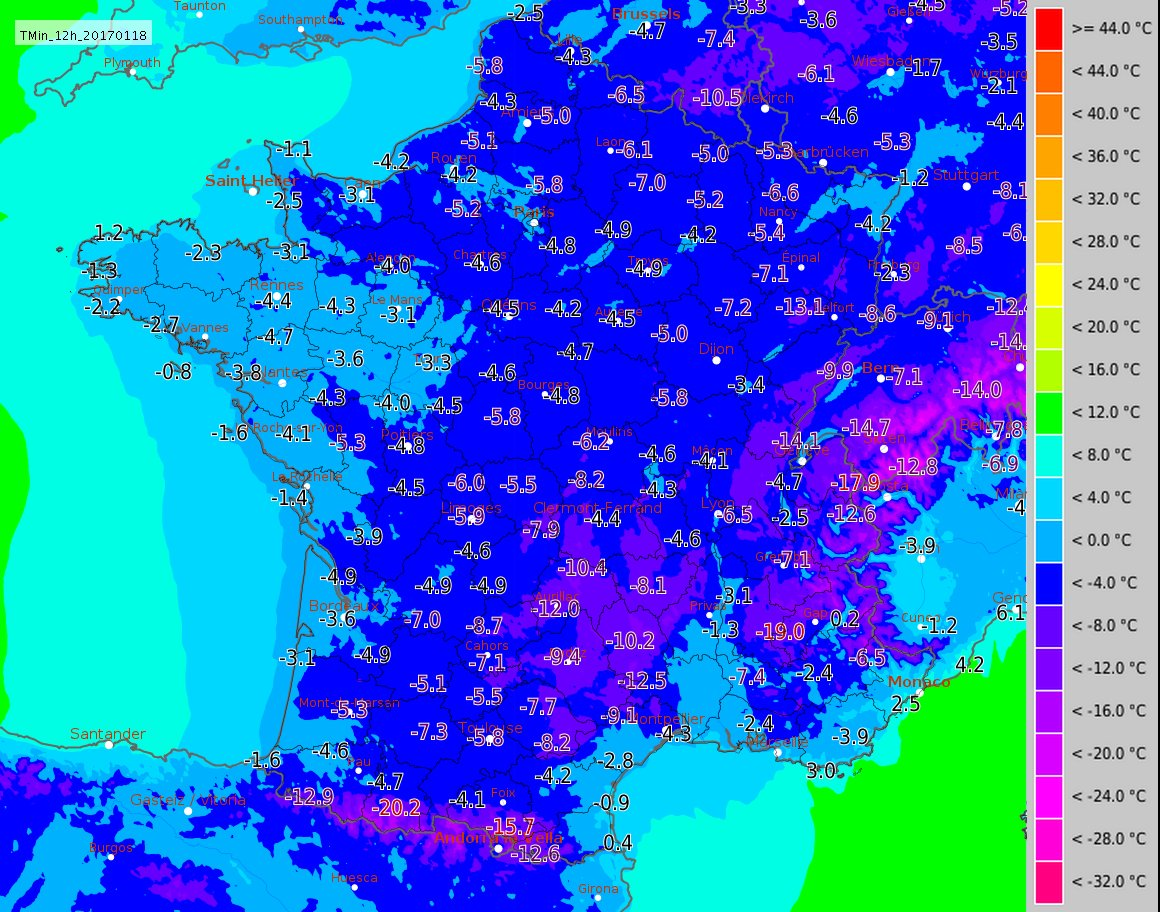
\includegraphics[width=\textwidth,height=0.8\textheight,keepaspectratio]{fig/meteo_fr_scales_temp}
  \end{figure}

\end{frame}

\begin{frame} \frametitle{}

  \begin{overprint}

    \onslide<1> \begin{figure}
      \centering
      \includegraphics[width=\textwidth,height=0.8\textheight,keepaspectratio]{fig/temp1}
      \caption{Température pour l'heure 1}
    \end{figure}

    \onslide<2> \begin{figure}
      \centering
      \includegraphics[width=\textwidth,height=0.8\textheight,keepaspectratio]{fig/temp2}
      \caption{Température pour l'heure 2}
    \end{figure}

    \onslide<3> \begin{figure}
      \centering
      \includegraphics[width=\textwidth,height=0.8\textheight,keepaspectratio]{fig/temp3}
      \caption{Température pour l'heure 3}
    \end{figure}

    \onslide<4> \begin{figure}
      \centering
      \includegraphics[width=\textwidth,height=0.8\textheight,keepaspectratio]{fig/temp4}
      \caption{Température pour l'heure 4}
    \end{figure}

    \onslide<5> \begin{figure}
      \centering
      \includegraphics[width=\textwidth,height=0.8\textheight,keepaspectratio]{fig/temp5}
      \caption{Température pour l'heure 5}
    \end{figure}

    \onslide<6> \begin{figure}
      \centering
      \includegraphics[width=\textwidth,height=0.8\textheight,keepaspectratio]{fig/temp6}
      \caption{Température pour l'heure 6}
    \end{figure}

  \end{overprint}

\end{frame}


\section[Isovaleurs]{Lignes iso-valeurs}

\begin{frame}
  \frametitle{Génération des lignes iso-valeurs}
  \begin{block}{Titre d'un bloc}
    \begin{itemize}
      \item Un point d'un bloc
    \end{itemize}
    Texte standard
  \end{block}



    \begin{overlayarea}{6cm}{1cm}
  \only<1>{\texttt{première idée overlayarea}}
  \only<2>{\texttt{deuxième idée overlayarea}}
  \only<3>{\texttt{troisième idée}}
  \only<4>{dernière idée}
 \end{overlayarea}
\end{frame}

\begin{frame} \frametitle{}

  \begin{overprint}

    \onslide<1> \begin{figure}
      \centering
      \includegraphics[width=\textwidth,height=0.8\textheight,keepaspectratio]{fig/temp1}
      \caption{Température pour l'heure 1}
    \end{figure}

    \onslide<2> \begin{figure}
      \centering
      \includegraphics[width=\textwidth,height=0.8\textheight,keepaspectratio]{fig/temp2}
      \caption{Température pour l'heure 2}
    \end{figure}

    \onslide<3> \begin{figure}
      \centering
      \includegraphics[width=\textwidth,height=0.8\textheight,keepaspectratio]{fig/temp3}
      \caption{Température pour l'heure 3}
    \end{figure}

    \onslide<4> \begin{figure}
      \centering
      \includegraphics[width=\textwidth,height=0.8\textheight,keepaspectratio]{fig/temp4}
      \caption{Température pour l'heure 4}
    \end{figure}

    \onslide<5> \begin{figure}
      \centering
      \includegraphics[width=\textwidth,height=0.8\textheight,keepaspectratio]{fig/temp5}
      \caption{Température pour l'heure 5}
    \end{figure}

    \onslide<6> \begin{figure}
      \centering
      \includegraphics[width=\textwidth,height=0.8\textheight,keepaspectratio]{fig/temp6}
      \caption{Température pour l'heure 6}
    \end{figure}

  \end{overprint}

\end{frame}


\section[Lignes de courant]{Lignes de courant}

\begin{frame}
  \frametitle{Génération des lignes de courant}
  \begin{columns}[T,totalwidth=\textwidth] % option T for best results ?
  \begin{column}{5cm}
  \begin{block}{Colonne 1}
    Texte dans la\\
    colonne 1.
  \end{block}
  \end{column}

  \begin{column}{5cm}
  \begin{block}{Colonne 2}
    Texte dans la
    colonne 2 qui peut être
    plus long que dans la
    colonne 1.
  \end{block}
  \end{column}
 \end{columns}
\end{frame}



\section{Visualisation complète}

\begin{frame} \frametitle{}

  \begin{overprint}

    \onslide<1> \begin{figure}
      \centering
      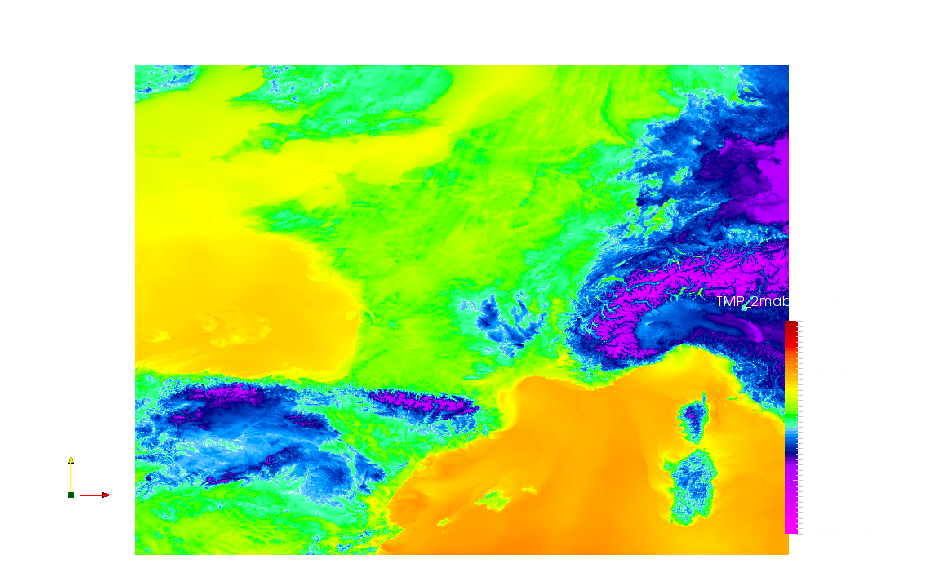
\includegraphics[width=\textwidth,height=0.8\textheight,keepaspectratio]{fig/1}
      \caption{Température pour l'heure 1}
    \end{figure}

    \onslide<2> \begin{figure}
      \centering
      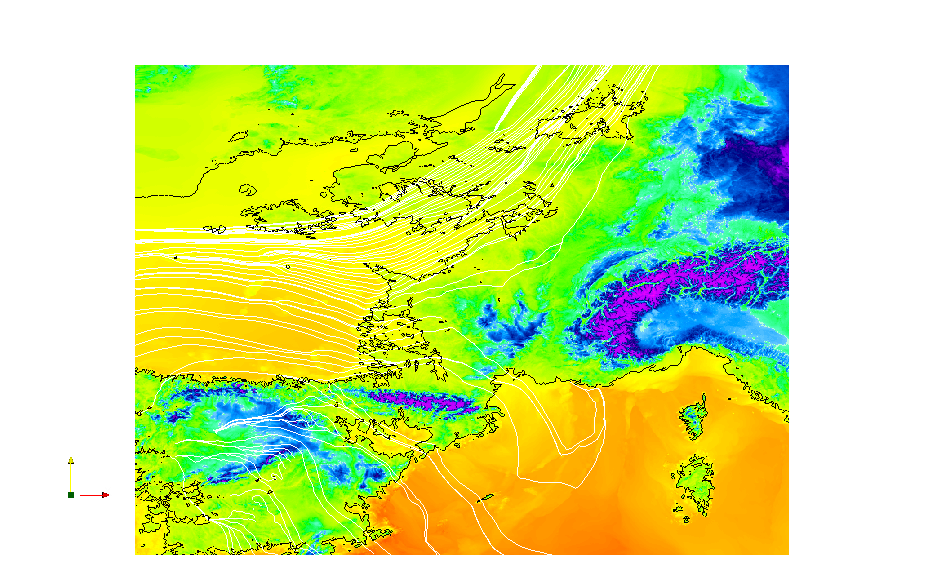
\includegraphics[width=\textwidth,height=0.8\textheight,keepaspectratio]{fig/2}
      \caption{Température pour l'heure 2}
    \end{figure}

    \onslide<3> \begin{figure}
      \centering
      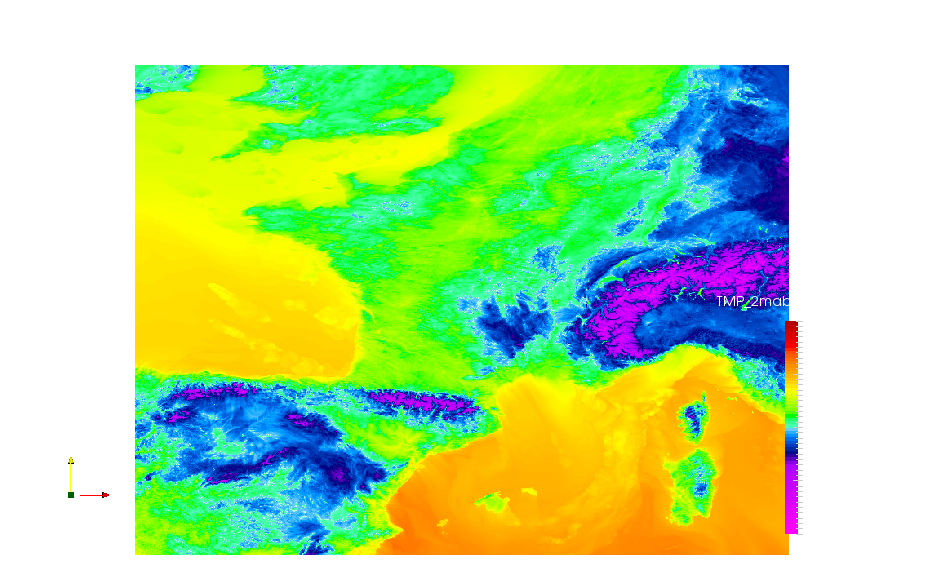
\includegraphics[width=\textwidth,height=0.8\textheight,keepaspectratio]{fig/3}
      \caption{Température pour l'heure 3}
    \end{figure}

    \onslide<4> \begin{figure}
      \centering
      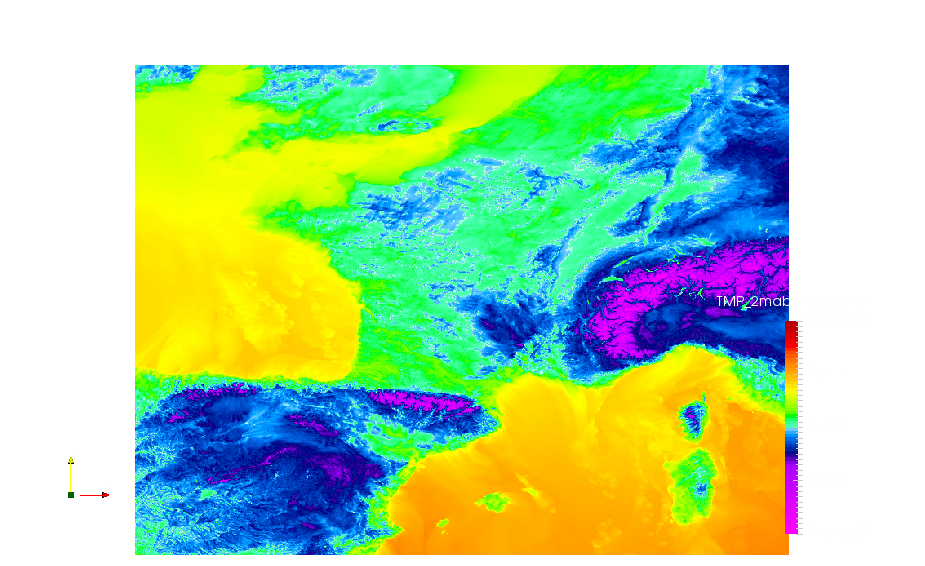
\includegraphics[width=\textwidth,height=0.8\textheight,keepaspectratio]{fig/4}
      \caption{Température pour l'heure 4}
    \end{figure}

    \onslide<5> \begin{figure}
      \centering
      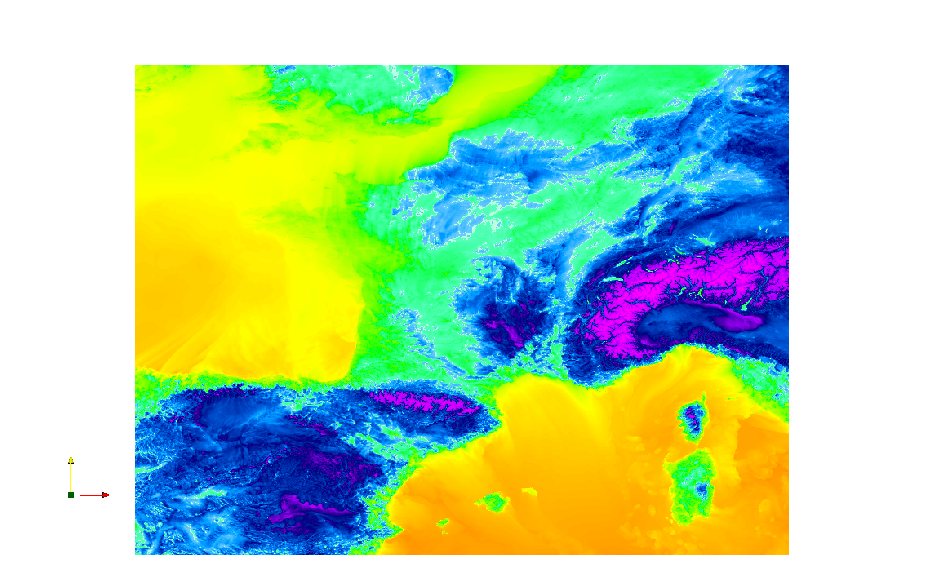
\includegraphics[width=\textwidth,height=0.8\textheight,keepaspectratio]{fig/5}
      \caption{Température pour l'heure 5}
    \end{figure}

    \onslide<6> \begin{figure}
      \centering
      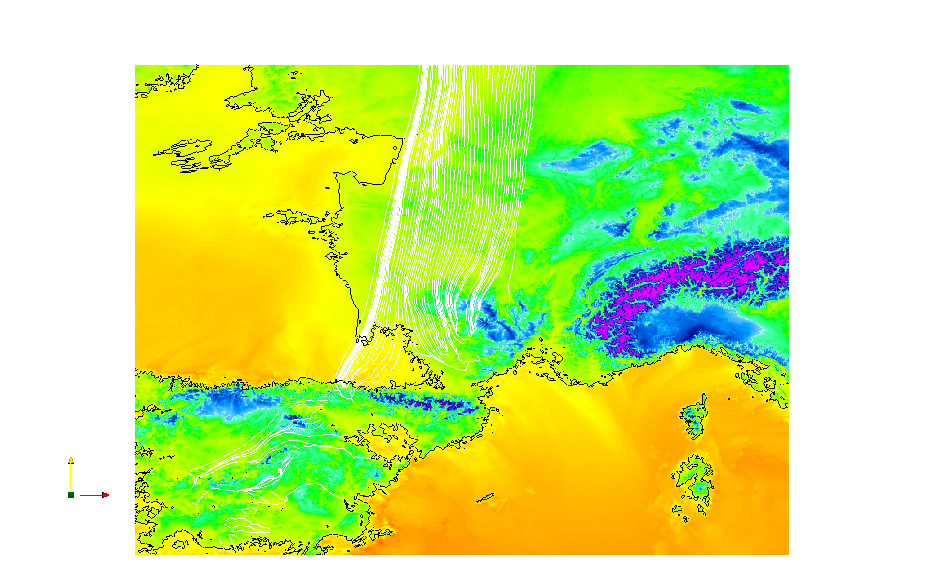
\includegraphics[width=\textwidth,height=0.8\textheight,keepaspectratio]{fig/6}
      \caption{Température pour l'heure 6}
    \end{figure}

  \end{overprint}

\end{frame}

\begin{frame}{}
  \centering
  Merci de votre attention
\end{frame}
\end{document}


%%% Local Variables:
%%% mode: latex
%%% TeX-master: t
%%% End:
